%==========================オプションおよび文書クラスの設定==========================
%"autodetect-engine"-どのエンジンでもコンパイル可能にするオプション
%"dvipdfmx-if-dvi"-必要な場合のみdvipdfmx経由のpdf化をするオプション(LuaTeXやXeTeXはPDFに直接変換するため)
%"ja=standard"-日本語文書の標準設定を利用するオプション
%"bxjs…"-どのエンジンでも利用可能なドキュメントクラス
%--以下のいずれかを選択--
\documentclass[autodetect-engine,dvipdfmx-if-dvi,ja=standard,a4paper,11pt]{bxjsarticle} %章の無いレポート
%\documentclass[autodetect-engine,dvipdfmx-if-dvi,ja=standard,a4paper,10pt]{bxjsslide} %スライド
%\documentclass[autodetect-engine,dvipdfmx-if-dvi,ja=standard,a4paper,10pt]{bxjsbook} %書籍
%\documentclass[autodetect-engine,dvipdfmx-if-dvi,ja=standard,a4paper,10pt]{bxjsreport} %章のある論文やレポート

%==============================プリアンブルの設定==============================
\title{研究会第2回} %タイトル
\author{B4 福田真悟} %著者名
\date{2020.5.12}%日付 %日付下の余白をN[mm]減らす

%///////////////////////////////////////////////////////////////////////////////////////////////////////////
%////////////////////////////////////パッケージの読込み及び設定の書換え//////////////////////////////////////
%///////////////////////////////////////////////////////////////////////////////////////////////////////////
\usepackage{graphicx} %図の挿入に関するパッケージ
\usepackage{float} %[H]で図の位置を固定する機能をONにするパッケージ
\usepackage{subcaption} %サブキャプションに関するパッケージ
\captionsetup{labelsep=space} %サブキャプション後の":"を非表示にする
\usepackage{enumerate} %{enumerate}[]の,[]の中の通りの箇条書きにすることができるパッケージ
\usepackage{amsmath} %数式に関するパッケージ
\usepackage{mathtools} %数式に関するパッケージ
\usepackage{bm} %ベクトル表示のコマンドを追加するパッケージ
\usepackage{comment} %複数行のコメントアウトを可能にするパッケージ
\usepackage{ascmac} %枠に関するパッケージ
\usepackage{tabularx} %表に関するパッケージ
\setpagelayout{top=10truemm,bottom=15truemm,left=15truemm,right=15truemm}  %余白に関する設定の書換え(bxjs…クラスではgeometryパッケージは使用不可)
\graphicspath{{../figures/}} %図を挿入する際に.texファイルの上の階層にあるfiguresというフォルダを参照可能にする
\usepackage{url}

%余白に関する設定の書換え(bxjs…クラスではgeometryパッケージは使用不可)
\belowcaptionskip=-0pt %キャプション下の余白をN[pt]減らす
\graphicspath{{../figures/}} %図を挿入する際に.texファイルの上の階層にあるfiguresというフォルダを参照可能にする

%使用記号の追加
\newcommand{\divergence}{\mathrm{div}\,}  %ダイバー
\newcommand{\grad}{\mathrm{grad}\,}  %グラディエント
\newcommand{\rot}{\mathrm{rot}\,}  %ローテーション

%\pagestyle{myheadings} %myheading文字列 emptyページ番号なし plainフッダーに
%\markright{\footnotesize 2月28日(金)15:00~ 顔合わせ}%全ページ共通への挿入
%================================以下本文================================
\begin{document}
\maketitle %設定したタイトルの挿入
\section{進捗状況}%sectionの前に*をつけると数字の振り分けが消える不思議
論文講読「Additive noise effects in active nonlinear spatially extended systems」\cite{all}\\
\ KS方程式のReservoir computingでの予測

\section{Noisy Kuramoto-Sivashinsky方程式}
まずモデルの概要図を下記に示す.
\begin{figure}[H]%[h]は記述したところ。[t]はそのページの上端。[t]はそのページの下端、[p]はページいっぱい
\begin{center}
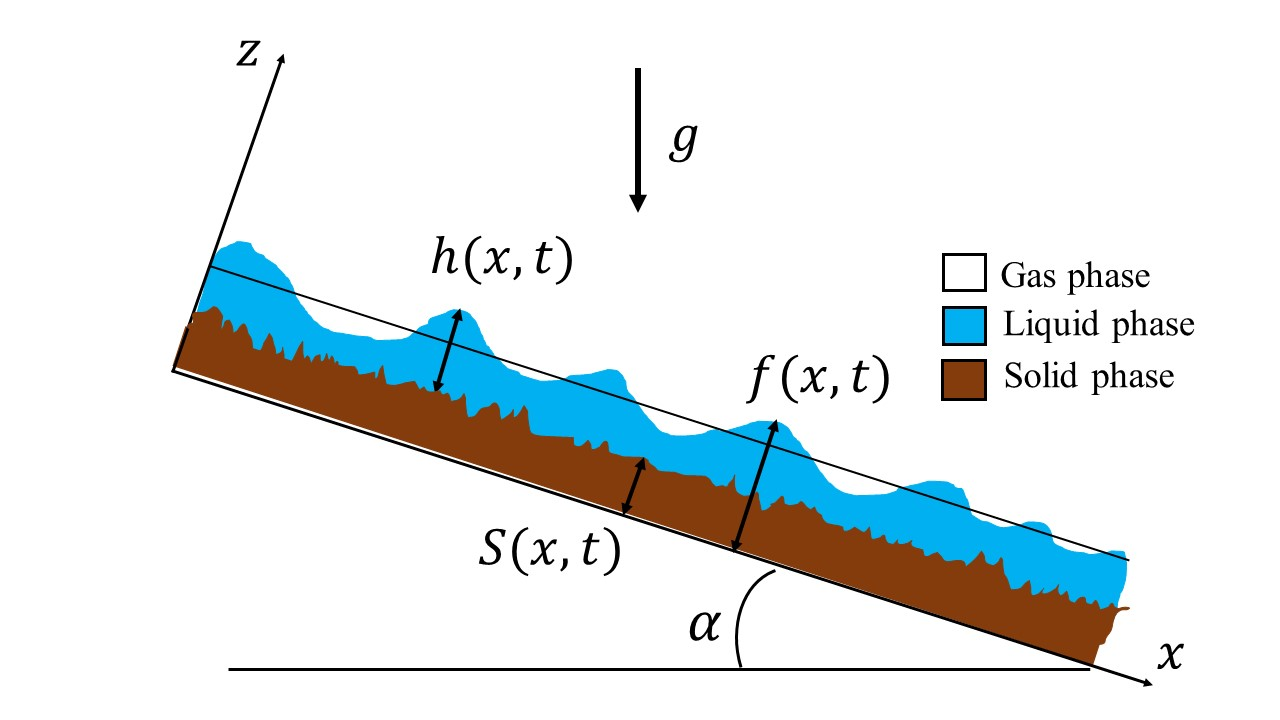
\includegraphics[width=.6\textwidth]{aboutNew.jpg} 
\end{center}
\caption{凹凸のある斜面に沿った液膜流の概要図}%図名
\label{fig:about}%fig図tb表
\end{figure}
図\ref{fig:about}に示す角度$\alpha$に傾いた凹凸のある斜面の上に流れる非常に薄く,レイノルズ数の小さい速度が遅い液膜流について考える.ここでの薄いは,流れのスケール($x$方向の長さ)に対して十分に無視できる厚さであり,レイノルズ数は${\rm Re}\ll1$とする.$h_0$を流れに乱れが生じなかった場合の膜厚で代表長さとする.$h(x,t),s(x,t),f(x,t)$はそれぞれ,個体壁,流れている液体,その和の厚さを示している.この液膜流に関しての1次元発展方程式を下記に示す.
\begin{equation}
U_T+UU_X\pm{U_{XX}}+U_{XXXX}=S(X,T)
\label{eq:nks}
\end{equation}
この方程式をNoisy Kuramoto-Sivashinsky方程式と呼ぶ.この式(\ref{eq:nks})の導出を下記にまとめる.


\subsection{Navier-Stokes方程式,連続の式の無次元化}
まず2次元Navier-Stokes方程式と連続の式を下記に示す.
\begin{subequations}
\begin{align}
\rho \left(\frac{\partial u}{\partial t}+u\frac{\partial u}{\partial x}+v\frac{\partial u}{\partial z}\right)&=-\frac{\partial p}{\partial x}+\mu \left(\frac{\partial ^2u}{\partial x^2}+\frac{\partial^2 u}{\partial z^2}\right)+\rho g\sin\alpha\label{eq:ns1}\\
\rho \left(\frac{\partial v}{\partial t}+u\frac{\partial v}{\partial x}+v\frac{\partial v}{\partial z}\right)&=-\frac{\partial p}{\partial z}+\mu \left(\frac{\partial ^2v}{\partial x^2}+\frac{\partial ^2v}{\partial z^2}\right)-\rho g\cos\alpha\label{eq:ns2}\\
\frac{\partial u}{\partial x}+\frac{\partial v}{\partial z}&=0\label{eq:mass}
\end{align}
\label{eq:ns}
\end{subequations}
このときの$(x,z,t)$はそれぞれの位置と時間を表し,$(u,v)$は$(x,z)$それぞれの方向の速度を表している.$\rho$は液体の密度,$\mu$は粘性係数,$p$は圧力を表している.また,重力加速度を$g$とする.\\
\ 次に無次元化を行うための代表パラメータを決定する.まず代表速度$U_0$について,液膜の表面速度を用いる.$s(x,t)=0$としたクエット流の場合のナビエストークス方程式は下記のようになる.
\begin{equation}
\begin{split}
0=\mu\frac{\partial^2 u}{\partial z^2}+\rho g\sin\alpha\\
\end{split}
\end{equation}
ここで境界条件を下記のようにする.
\begin{equation}
\begin{split}
z&=0\ \rightarrow\ u=0\\
z&=h(x,t)\ \rightarrow\ 
\frac{\partial u}{\partial z}=0\\
\end{split}
\end{equation}
このときの表面における流体の速度は,
\begin{equation}
U_0=\frac{\rho gh_0^2\sin\alpha}{2\mu}
\end{equation}
となる.この値を代表速度とする.代表時間は$T_0=h_0/U_0$,代表圧力は粘性係数に速度勾配をかけた$P_0=\mu U_0/h_0$とする.\\
\ 無次元化したパラメータを下記に示す.
\begin{equation}
\begin{split}
x^*=\frac{x}{h_0},z^*=\frac{z}{h_0},u^*=\frac{u}{U_0}\\
v^*=\frac{v}{U_0},t^*=\frac{t}{T_0},p^*=\frac{p}{P_0}\\
\end{split}
\end{equation}
無次元数として,慣性力と粘性力との比を表すレイノルズ数${\rm Re}=\rho U_0h_0/\mu$と粘性力と表面張力$\gamma$の比を表すキャピラリー数${\rm Ca}=\mu U_0/\gamma$を用いる.式(\ref{eq:ns})を無次元化したものを下記に示す.\\
式(\ref{eq:ns1})$\Leftrightarrow$
\begin{equation*}
\begin{split}
&\rho\frac{U_0^2}{h_0}\left(\frac{\partial u^*}{\partial t^*}+u^*\frac{\partial u^*}{\partial x^*}+v^*\frac{\partial u^*}{\partial z^*}\right)=-\frac{\mu U_0}{h_0^2}\frac{\partial p^*}{\partial x^*}+\frac{\mu U_0}{h_0^2}\left(\frac{\partial ^2u^*}{\partial x^{*2}}+\frac{\partial^2 u^*}{\partial z^{*2}}\right)+\rho g\sin\alpha\\
\Leftrightarrow&\frac{U_0^2}{h_0}\frac{2}{g\sin\alpha}\left(\frac{\partial u^*}{\partial t^*}+u^*\frac{\partial u^*}{\partial x^*}+v^*\frac{\partial u^*}{\partial z^*}\right)=-\frac{\mu U_0}{h_0^2}\frac{2}{\rho g\sin\alpha}\frac{\partial p^*}{\partial x^*}+\frac{\mu U_0}{h_0^2}\frac{2}{\rho g\sin\alpha}\left(\frac{\partial ^2u^*}{\partial x^{*2}}+\frac{\partial^2 u^*}{\partial z^{*2}}\right)+2\\
\Leftrightarrow&{\rm Re}\left(\frac{\partial u^*}{\partial t^*}+u^*\frac{\partial u^*}{\partial x^*}+v^*\frac{\partial u^*}{\partial z^*}\right)=-\frac{\partial p^*}{\partial x^*}+\left(\frac{\partial ^2u^*}{\partial x^{*2}}+\frac{\partial^2 u^*}{\partial z^{*2}}\right)+2
\end{split}
\end{equation*}
式(\ref{eq:ns2})$\Leftrightarrow$
\begin{equation*}
\begin{split}
&\rho\frac{U_0^2}{h_0}\left(\frac{\partial v^*}{\partial t^*}+u^*\frac{\partial v^*}{\partial x^*}+v^*\frac{\partial v^*}{\partial z^*}\right)=-\frac{\mu U_0}{h_0^2}\frac{\partial p^*}{\partial z^*}+\frac{\mu U_0}{h_0^2}\left(\frac{\partial ^2v^*}{\partial x^{*2}}+\frac{\partial ^2v^*}{\partial z^{*2}}\right)-\rho g\cos\alpha\\
\Leftrightarrow&\frac{U_0^2}{h_0}\frac{2}{g\sin\alpha}\left(\frac{\partial v^*}{\partial t^*}+u^*\frac{\partial v^*}{\partial x^*}+v^*\frac{\partial v^*}{\partial z^*}\right)=-\frac{\mu U_0}{h_0^2}\frac{2}{\rho g\sin\alpha}\frac{\partial p^*}{\partial z^*}+\frac{\mu U_0}{h_0^2}\frac{2}{\rho g\sin\alpha}\left(\frac{\partial ^2v^*}{\partial x^{*2}}+\frac{\partial ^2v^*}{\partial z^{*2}}\right)-2\cot\alpha\\
\Leftrightarrow&{\rm Re}\left(\frac{\partial v^*}{\partial t^*}+u^*\frac{\partial v^*}{\partial x^*}+v^*\frac{\partial v^*}{\partial z^*}\right)=-\frac{\partial p^*}{\partial z^*}+\left(\frac{\partial ^2v^*}{\partial x^{*2}}+\frac{\partial ^2v^*}{\partial z^{*2}}\right)-2\cot\alpha
\end{split}
\end{equation*}
式(\ref{eq:mass})$\Leftrightarrow$
\begin{equation*}
\frac{\partial u^*}{\partial x^*}+\frac{\partial v^*}{\partial z^*}=0
\end{equation*}
以上の計算結果を下記にまとめる.便宜上,無次元化された関数$(u,v,p)$の$x$方向の1階微分をそれぞれ$(u_x,v_x,p_x)$とし,2階微分以降は$u_{xx}$のように増えて記述する.$z,t$方向も同様である.
\begin{subequations}
\begin{align}
{\rm Re}(u_t+uu_x+vu_z)&=-p_x+u_{xx}+u_{zz}+2\label{eq:gns1}\\
{\rm Re}(v_t+uv_x+vv_z)&=-p_z+v_{xx}+v_{zz}-2\cot\alpha\label{eq:gns2}\\
u_x+v_z&=0\label{eq:gmass}
\end{align}
\label{eq:gns}
\end{subequations}

\subsection{液膜流の境界条件}
液膜流の境界条件について考える.まず個体壁の接触している$z=s(x,t)$の境界条件は,個体壁は$x$方向には動かず,$z$方向に$s_t(x,t)$の速度で変位する.個体壁との相対速度は0となるので,各方向速度の境界条件は,
\begin{subequations}
\begin{align}
z&=s(x,t)\ \rightarrow\ u=0\label{eq:sbc1}\\
z&=s(x,t)\ \rightarrow\ v=s_t(x,t)\label{eq:sbc2}
\end{align}
\label{eq:sbc}
\end{subequations}
となる.\\
\ 次に自由表面の$z=f(x,t)$の境界条件について考える.自由表面の境界条件は運動学的条件,応力境界条件(垂直方向と剪断方向)の3つである.運動学的条件は,自由表面上の流体粒子は常に自由表面と同じ動きをするという境界条件である.自由表面上の流体粒子の速度$v$と自由表面の時間変化$Df/Dt$が等しいので,
\begin{equation*}
\begin{split}
&v=\frac{Df(x,t)}{Dt}=f_t+uf_x\\
\Leftrightarrow&f_t+uf_x-v=0
\end{split}
\end{equation*}
となる.最後の応力境界条件は,自由表面での剪断応力は,空気の粘性が液体の粘性よりの十分小さいことから0となり,垂直応力は,圧力と表面張力と等しくなるという境界条件である.通常の$(x,z)$座標系での応力テンソルでは,変位で傾きのある流れの自由表面の垂直応力,剪断応力がわからない.そこで,自由表面の傾き$\theta$に合わせて,$\theta$傾いた座標系$(x',z')$を用いる.このときの傾きは,$\tan\theta=f_x$となる.自由表面の応力テンソルとの変換の詳細を下記の図\ref{fig:sigma}に示す.
\begin{figure}[H]%[h]は記述したところ。[t]はそのページの上端。[t]はそのページの下端、[p]はページいっぱい
\begin{center}
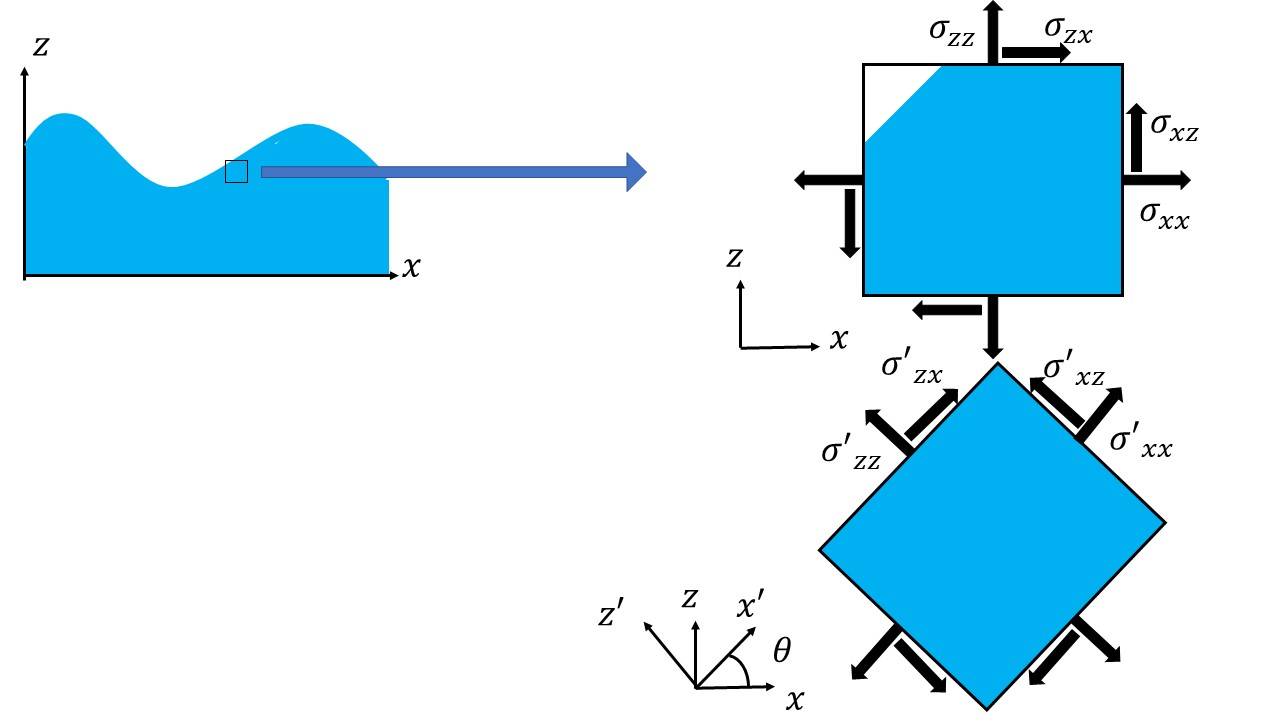
\includegraphics[width=.6\textwidth]{sigma.jpg} 
\end{center}
\caption{自由表面の応力テンソルの変換}%図名
\label{fig:sigma}%fig図tb表
\end{figure}
応力テンソルは,流体の粘性による応力となるので
\begin{equation}
{\boldsymbol \sigma} = \left[
\begin{array}{ccc}
\sigma_{xx} & \sigma_{xz}\\
\sigma_{zx} & \sigma_{zz}
\end{array}
\right]= \left[
\begin{array}{ccc}
2\mu U_0u_x & \mu U_0\left(u_z+v_x\right)\\
\mu U_0\left(u_z+v_x\right) & 2\mu U_0v_z
\end{array}
\right]
\end{equation}
と表される.コーシーの公式を用いて変換した座標の応力テンソル${\boldsymbol \sigma'}$を$\theta$の回転行列${\boldsymbol Q}$を用いて下記に示す.
\begin{equation}
{\boldsymbol \sigma'}={\boldsymbol Q}{\boldsymbol\sigma}{\boldsymbol Q^{\mathrm{T}}}=\left[
\begin{array}{ccc}
\cos\theta & \sin\theta\\
-\sin\theta & \cos\theta
\end{array}
\right]\left[
\begin{array}{ccc}
\sigma_{xx} & \sigma_{xz}\\
\sigma_{zx} & \sigma_{zz}
\end{array}
\right]\left[
\begin{array}{ccc}
\cos\theta & -\sin\theta\\
\sin\theta & \cos\theta
\end{array}
\right]
\end{equation}
変換後の$(\sigma'_{zx},\sigma'_{zz})$がそれぞれ条件から$(0,p-\gamma f_{xx}(1+f_x^2)^{-3/2})$となるので運動学的条件とまとめると,
\begin{subequations}
\begin{align}
z&=f(x,t)\ \rightarrow\ f_t+uf_x-v=0\label{eq:abc1}\\
z&=f(x,t)\ \rightarrow\ (1-f_x^2)(u_z+v_x)+2f_x(v_z-u_x)=0\label{eq:abc2}\\
z&=f(x,t)\ \rightarrow\ p=\frac{2}{1+f_x^2}(-f_x(u_z+v_x)+u_xf_x^2+v_z)-\frac{f_{xx}}{{\rm Ca}(1+f_x^2)^{3/2}}\label{eq:abc3}
\end{align}
\label{eq:abc}
\end{subequations}
となる.
\subsection{摂動法}
摂動法は,主要な力(主要項)による運動が他の副次的な力(摂動項)によって乱される現象に対して,摂動項を微小パラメータ$\varepsilon$を用いて,そのオーダーをわけて計算し,1次のオーダーが主要項にどのような影響を与えるのか調べる方法である.
\subsubsection{長波パラメータ$\varepsilon$}
今回の微小パラメータ$\varepsilon$は,液膜の厚さと$x$方向の変動が生じる長さスケールとの比で表される長波パラメータとする.新しい座標系の$(\xi,\tau)=(\varepsilon x,\varepsilon t)$を導入し,$z$方向速度は,微小となるので,$w=v/\varepsilon$とし,キャピラリー数も${\rm Ca}=O(\varepsilon^2)$のオーダーと推定できるので,$\tilde{\rm Ca}={\rm Ca}/\varepsilon^2$とする.$(\xi,z)$方向の速度$(u,w)$と圧力は,それぞれ$\varepsilon$で級数展開し,$u=u_0+\varepsilon u_1+\cdots,w=w_0+\varepsilon w_1+\cdots,p=p_0+\varepsilon p_1+\cdots$とする.これによって,摂動項の影響と主要項の影響を分解して考えることができる.変数変換した式(\ref{eq:gns}),式(\ref{eq:sbc}),式(\ref{eq:abc})を下記に示す.
\begin{subequations}
\begin{align}
\varepsilon{\rm Re}(u_\tau+uu_\xi+wu_z)&=-\varepsilon p_\xi+\varepsilon^2u_{\xi\xi}+u_{zz}+2\label{eq:egns1}\\
\varepsilon^2{\rm Re}(w_\tau+uw_\xi+ww_z)&=-p_z+\varepsilon^2w_{\xi\xi}+\varepsilon w_{zz}-2\cot\alpha\label{eq:egns2}\\
u_\xi+w_z&=0\label{eq:egmass}
\end{align}
\label{eq:egns}
\end{subequations}
\begin{subequations}
\begin{align}
z&=s(\xi,\tau)\ \rightarrow\ u=0\label{eq:esbc1}\\
z&=s(\xi,\tau)\ \rightarrow\ w=s_\tau(\xi,\tau)\label{eq:esbc2}
\end{align}
\label{eq:esbc}
\end{subequations}
\begin{subequations}
\begin{align}
z&=f(\xi,\tau)\ \rightarrow\ f_\tau+uf_\xi-w=0\label{eq:eabc1}\\
z&=f(\xi,\tau)\ \rightarrow\ (1-\varepsilon^2f_\xi^2)(u_z+\varepsilon^2w_\xi)+2\varepsilon^2f_\xi(w_z-u_\xi)=0\label{eq:eabc2}\\
z&=f(\xi,\tau)\ \rightarrow\ p=\frac{2}{1+\varepsilon^2f_\xi^2}(-\varepsilon f_\xi(u_z+\varepsilon^2w_\xi)+\varepsilon^3u_\xi f_\xi^2+\varepsilon w_z)-\frac{f_{\xi\xi}}{\tilde{\rm Ca}(1+\varepsilon^2f_\xi^2)^{3/2}}\label{eq:eabc3}
\end{align}
\label{eq:eabc}
\end{subequations}
\subsubsection{$\varepsilon$の0次オーダー}
まず$\varepsilon$の0次オーダーで主要項について考える.級数展開を考慮し,$\varepsilon$の0次のみを残した式(\ref{eq:egns})$\sim$式(\ref{eq:eabc})を下記に示す.
\begin{subequations}
\begin{align}
0&=u_{0zz}+2\label{eq:0egns1}\\
0&=-p_{0z}-2\cot\alpha\label{eq:0egns2}\\
u_{0\xi}+w_{0z}&=0\label{eq:0egmass}
\end{align}
\label{eq:0egns}
\end{subequations}
\begin{subequations}
\begin{align}
z&=s(\xi,\tau)\ \rightarrow\ u_0=0\label{eq:0esbc1}\\
z&=s(\xi,\tau)\ \rightarrow\ w_0=s_\tau(\xi,\tau)\label{eq:0esbc2}
\end{align}
\label{eq:0esbc}
\end{subequations}
\begin{subequations}
\begin{align}
z&=f(\xi,\tau)\ \rightarrow\ f_\tau+uf_\xi-w=0\label{eq:0eabc1}\\
z&=f(\xi,\tau)\ \rightarrow\ u_{0z}=0\label{eq:0eabc2}\\
z&=f(\xi,\tau)\ \rightarrow\ p_0=-\frac{f_{\xi\xi}}{\tilde{\rm Ca}}\label{eq:0eabc3}
\end{align}
\label{eq:0eabc}
\end{subequations}
上記の式(\ref{eq:0egns})$\sim$式(\ref{eq:0eabc})の中で式(\ref{eq:0eabc1})を除くすべての式を用いると,$u_0,w_0,p_0$はそれぞれ下記の式となる.
\begin{subequations}
\begin{align}
u_0&=-(z-h-s)^2+h^2\label{eq:u0}\\
w_0&=u_0(h+s)_\xi-[h^2]_\xi(z-s)+s_\tau\label{eq:v0}\\
p_0&=-2(\cot\alpha)(z-h-s)-\frac{(h+s)_{\xi\xi}}{\tilde{\rm Ca}}\label{eq:p0}
\end{align}
\label{eq:all0}
\end{subequations}
\ 次に式(\ref{eq:0eabc1})を用いて質量保存則を導出する.まず連続の式である式(\ref{eq:egmass})を$z$方向に積分したものを下記に示す.
\begin{equation}
\int^{f(\xi,\tau)}_{s(\xi,\tau)}u_\xi\ dz+w(\xi,f,\tau)-w(\xi,s,\tau)=0\label{eq:zmass}
\end{equation}
この式を境界条件の式(\ref{eq:0eabc1})から,$w(\xi,f,\tau)=f_\tau+u(\xi,f,\tau)f_\xi$,式(\ref{eq:esbc2})から$w(\xi,s,\tau)=s_\tau$となることがわかる.残りの$\xi$方向微分の項は,一般化されたLeibnizの積分公式から,
\begin{equation}
\int^{f}_{s}u_\xi\ dz=\frac{d}{d\xi}\int^{f}_{s}u\ dz-f_\xi u(\xi,f,\tau)+s_\xi u(\xi,s,\tau)\label{eq:leibniz}
\end{equation}
式(\ref{eq:esbc1})から$u(\xi,s,\tau)=0$となる.ここで流量を定義する.流量は$x$方向速度である$u$の$z$方向に積分した値となる.流量$q$を表す式を下記に示す.
\begin{equation}
q=\int^{f}_{s}u\ dz\label{eq:q}
\end{equation}
式(\ref{eq:leibniz})と式(\ref{eq:q})を式(\ref{eq:zmass})に代入したものを下記に示す.
\begin{equation}
h_\tau+q_\xi=0\label{eq:tmass}
\end{equation}
\ ここで流量$q$について,他の値と同様に級数展開し,$q=q_0+\varepsilon q_1+\cdots$とし,式(\ref{eq:u0})から0次オーダーの$x$方向速度$u_0$が関数としてわかっているのでそれを式(\ref{eq:q})に代入したものを下記に示す.
\begin{equation}
\begin{split}
q_0&=\int^{f}_{s}-(z-h-s)^2+h^2\ dz\\
&=\frac{2}{3}h^3
\label{eq:q0}
\end{split}
\end{equation}
この値を式(\ref{eq:tmass})に代入したものを下記に示す.
\begin{equation}
h_\tau+\left[\frac{2}{3}h^3\right]_\xi+O(\varepsilon)=0\label{eq:qtmass}
\end{equation}
\subsubsection{$\varepsilon$の1次オーダー}
次は,$\varepsilon$の1次オーダーで摂動項について考える.級数展開を考慮し,$\varepsilon$の1次のみを残した式(\ref{eq:egns})$\sim$式(\ref{eq:eabc})を下記に示す.また,式(\ref{eq:eabc1})は,質量保存則によって常に成立するので今回は省略する.
\begin{subequations}
\begin{align}
{\rm Re}(u_{0\tau}+u_0u_{0\xi}+w_0u_{0z})&=-p_{0\xi}+u_{1zz}\label{eq:1egns1}\\
0&=-p_{1z}+w_{0zz}\label{eq:1egns2}\\
u_{1\xi}+w_{1z}&=0\label{eq:1egmass}
\end{align}
\label{eq:1egns}
\end{subequations}
\begin{subequations}
\begin{align}
z&=s(\xi,\tau)\ \rightarrow\ u_1=0\label{eq:1esbc1}\\
z&=s(\xi,\tau)\ \rightarrow\ w_1=0\label{eq:1esbc2}
\end{align}
\label{eq:1esbc}
\end{subequations}
\begin{subequations}
\begin{align}
z&=f(\xi,\tau)\ \rightarrow\ u_{1z}=0\label{eq:1eabc2}\\
z&=f(\xi,\tau)\ \rightarrow\ p_1=2(-f_\xi u_{0z}+w_{0z})\label{eq:1eabc3}
\end{align}
\label{eq:1eabc}
\end{subequations}
上記の式(\ref{eq:1egns})$\sim$式(\ref{eq:1eabc})から$u_1$は下記の式となる.
\begin{equation}
\begin{split}
u_1=&{\rm Re}\left[\frac{1}{6}hh_\xi(z-h-s)^4+\frac{1}{3}(h_\tau+2h^2h_\xi)(z-h-s)^3+(hh_\tau+h^3h_\xi)(z-h-s)^2\right]\\
&+\frac{1}{2}\left(2(\cot\alpha)(h+s)_\xi-\frac{(h+s)_{\xi\xi\xi}}{\tilde{\rm Ca}}\right)[(z-h-s)^2-h^2]-{\rm Re}\left[\frac{1}{2}h^5h_\xi+\frac{2}{3}h^3h_\tau\right]
\end{split}
\end{equation}
次に流量$q_1$を求めるために$u_1$を式(\ref{eq:q})に代入したものを下記に示す.
\begin{equation}
\begin{split}
q_1=\int^{f}_{s}u\ dz={\rm Re}\left[-\frac{3}{10}h^6h_\xi-\frac{5}{12}h^4h_\tau\right]-\frac{1}{3}h^3\left(2(\cot\alpha)(h+s)_\xi-\frac{(h+s)_{\xi\xi\xi}}{\tilde{\rm Ca}}\right)
\end{split}
\label{eq:q1}
\end{equation}
ここで0次オーダーの保存式(\ref{eq:tmass})から$h_\tau=-\left[\frac{2}{3}h^3\right]_\xi-O(\varepsilon)=-2h^2h_\xi$となることがわかる.この式を式(\ref{eq:q1})に代入したものを下記に示す.
\begin{equation}
\begin{split}
q_1=h^3\left[\frac{8{\rm Re}}{15}h^3h_\xi-\frac{2}{3}(\cot\alpha)(h+s)_\xi+\frac{1}{3}\frac{(h+s)_{\xi\xi\xi}}{\tilde{\rm Ca}}\right]
\end{split}
\label{eq:q1h}
\end{equation}
流量を$q=q_0+\varepsilon q_1$とし,保存式(\ref{eq:tmass})に代入したものを下記に示す.
\begin{equation}
h_\tau+\left(\frac{2}{3}h^3+\varepsilon h^3\left[\frac{8{\rm Re}}{15}h^3h_\xi-\frac{2}{3}(\cot\alpha)(h+s)_\xi+\frac{1}{3}\frac{(h+s)_{\xi\xi\xi}}{\tilde{\rm Ca}}\right]\right)_\xi=0\label{eq:q1mass}
\end{equation}
\subsection{変数変換と整理}
式(\ref{eq:q1mass})の$h=1+\varepsilon\eta,s=\varepsilon\sigma$とし,新しい座標系$(\chi,\tilde{\tau})=(\xi-2\tau,\varepsilon\tau)$でガリレイ変換を行う.ガリレイ変換の微分式を下記に示す.
\begin{equation}
\begin{split}
\eta_\tau&=\bar{\eta}_\chi\frac{\partial\chi}{\partial\tau}+\bar{\eta}_{\tilde{\tau}}\frac{\partial\tilde{\tau}}{\partial\tau}=-2\bar{\eta}_\chi+\varepsilon\bar{\eta}_{\tilde{\tau}}\\
\eta_\xi&=\bar{\eta}_\chi\frac{\partial\chi}{\partial\xi}+\bar{\eta}_{\tilde{\tau}}\frac{\partial\tilde{\tau}}{\partial\xi}=\bar{\eta}_\chi\\
\eta_{\xi\xi\cdots}&=\bar{\eta}_{\chi\chi\cdots}
\label{eq:gari}
\end{split}
\end{equation}
以上の式を代入し,$\varepsilon$の0次オーダーをとったものを下記に示す.
\begin{equation*}
\begin{split}
&\varepsilon\eta_\tau+\left(\frac{2}{3}(1+3\varepsilon\eta+3\varepsilon^2\eta^2)+\varepsilon^2 \left[\frac{8{\rm Re}}{15}\eta_\xi-\frac{2}{3}(\cot\alpha)(\eta+\sigma)_\xi+\frac{1}{3}\frac{(\eta+\sigma)_{\xi\xi\xi}}{\tilde{\rm Ca}}\right]\right)_\xi=0\\
\Leftrightarrow&\eta_\tau+(2\eta_\xi+4\varepsilon\eta\eta_\xi)+\varepsilon \left[\frac{8{\rm Re}}{15}\eta_{\xi\xi}-\frac{2}{3}(\cot\alpha)(\eta+\sigma)_{\xi\xi}+\frac{1}{3}\frac{(\eta+\sigma)_{\xi\xi\xi\xi}}{\tilde{\rm Ca}}\right]=0\\
\mbox{式(\ref{eq:gari})のガリレイ変換より}\\
\Leftrightarrow&\varepsilon\bar{\eta}_{\tilde{\tau}}+4\varepsilon\bar{\eta}\bar{\eta}_\chi+\varepsilon \left[\frac{8{\rm Re}}{15}\bar{\eta}_{\chi\chi}-\frac{2}{3}(\cot\alpha)(\bar{\eta}+\bar{\sigma})_{\chi\chi}+\frac{1}{3}\frac{(\bar{\eta}+\bar{\sigma})_{\chi\chi\chi\chi}}{\tilde{\rm Ca}}\right]=0\\
\end{split}
\end{equation*}
この式をノイズ項($\tau$)を分け,右辺にまとめたものを下記に示す.
\begin{equation}
\bar{\eta}_{\tilde{\tau}}+4\bar{\eta}\bar{\eta}_\chi+\left(\frac{8{\rm Re}}{15}-\frac{2\cot\alpha}{3}\right)\bar{\eta}_{\chi\chi}+\frac{1}{3\tilde{\rm Ca}}\bar{\eta}_{\chi\chi\chi\chi}=\frac{2\cot\alpha}{3}\bar{\sigma}_{\chi\chi}-\frac{1}{3\tilde{\rm Ca}}\bar{\sigma}_{\chi\chi\chi\chi}\label{eq:kseta}
\end{equation}
係数が1となるように定数を設定した場合の簡略化された式を下記に示す.
\begin{equation}
U_T+UU_X\pm{U_{XX}}+U_{XXXX}=S(X,T)
\label{eq:nks1}
\end{equation}
この式は式(\ref{eq:nks})と一致する.


%\begin{figure}[H]%[h]は記述したところ。[t]はそのページの上端。[t]はそのページの下端、[p]はページいっぱい
%\begin{center}
%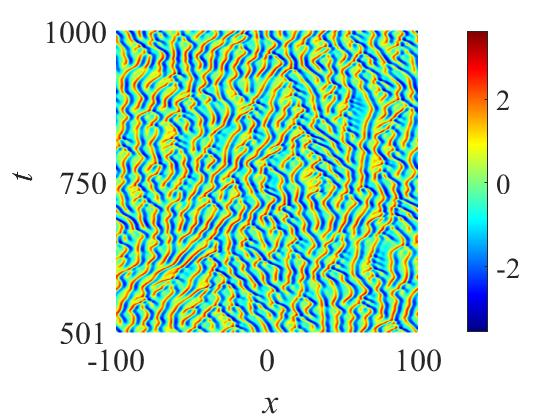
\includegraphics[width=.4\textwidth]{KS_result.jpg} 
%\end{center}
%\caption{KS方程式の結果}%図名
%\label{fig:ks}%fig図tb表
%\end{figure}

\newpage
\section{KS方程式のReservoir computingでの予測}
今回で用いた方程式は1D\ gKS方程式である.まず1D\ gKS方程式を下記に示す.
\begin{equation}
\frac{\partial u}{\partial t}+u\frac{\partial u}{\partial x}+\frac{\partial^2 u}{\partial x^2}+\delta\frac{\partial^3 u}{\partial x^3}+\nu\frac{\partial^4 u}{\partial x^4}=0
\label{eq:ks}
\end{equation}
今回のKS方程式でのパラメータを下記にまとめる.
\begin{itembox}[l]{KS方程式導出のパラメータ}
システムサイズ$L=-100\sim100$,刻み幅$dx=0.2$,刻み時間$dt=0.1$,時間$t=0\sim 10000$,$\delta=0$,$\nu=1.0$
\end{itembox}
\\
\ 次にスペクトル法によって導出されたKS方程式の解の最大値と最小値をそれぞれを$u_{max},u_{min}$とし,$-1\sim1$となるように入力正規化を行う.正規化された$u_{normal}$の導出方法を下記に示す.
\begin{equation}
u_{normal}=2\left(\frac{u-u_{min}}{u_{max}-u_{min}}-0.5\right)
\end{equation}
RCへと入力値を下記にまとめる.
\begin{itembox}[l]{入力されるKS方程式}
刻み幅$dx=1$ごとに並んだ入力値を用いる.\\
時間$dt=0.1$後を予測を行う.\\
入力値は$-1\sim1$に正規化された値を用いる.
\end{itembox}
\\
\ 最後にRCのパラメータを下記にまとめる.
\begin{itembox}[l]{RCのパラメータ}
学習回数97001回,初期のダイナミクスを除去するために最初の1000回は無視する.($t=0\sim100$)\\
出力回数1000回,入力層の数201個($L=-100\sim100$),出力層の数201個,中間層の数5000個\\
記憶力$\alpha=1.0$\\
入力層の重み$W_{in}$は,$-0.00258\sim0.00258$の一様分布\\
中間層の重み$W_{res}$は,$-0.000536\sim0.000536$の一様分布
\end{itembox}
\\
\ 以上のパラメータを用いて予測を行う.元の時系列データの$dt=0.1$刻みで$t=0\sim50$までの時空構造,RCで予測した出力の500回の時空構造,その2つの絶対誤差の時空構造の3つを下記に示す.
\begin{figure}[H]%[h]は記述したところ。[t]はそのページの上端。[t]はそのページの下端、[p]はページいっぱい
\begin{center}
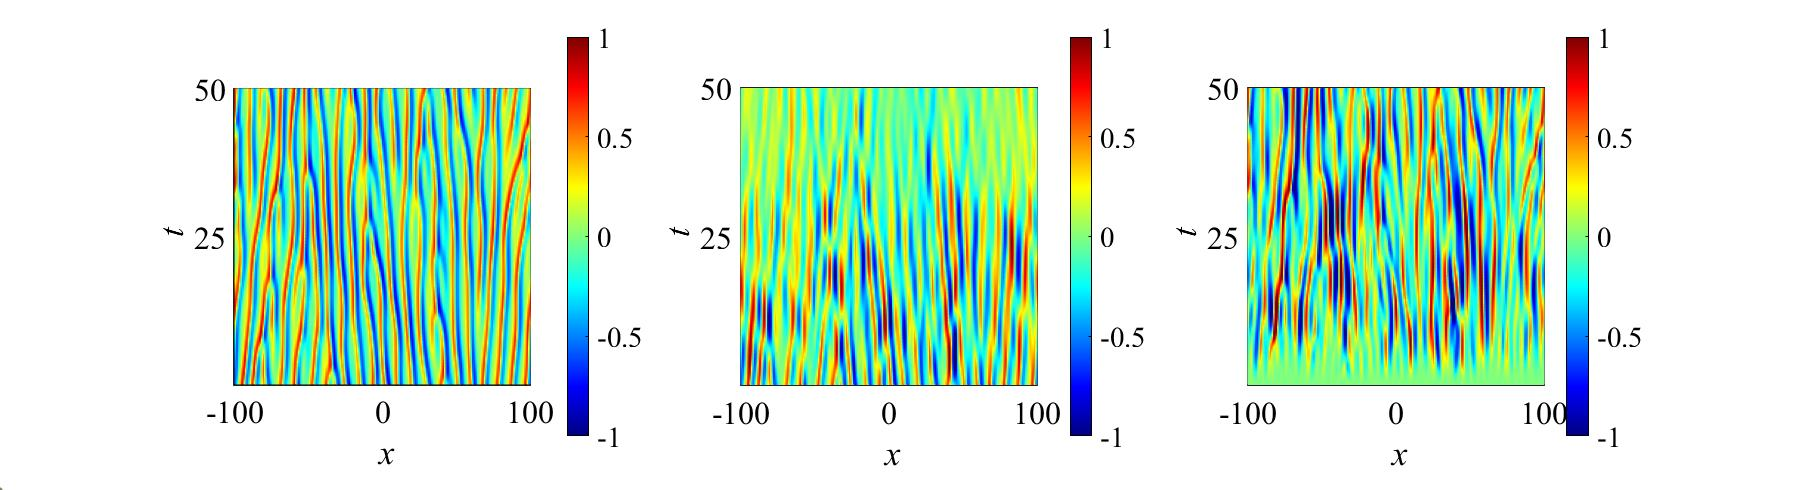
\includegraphics[width=.9\textwidth]{KS_error2.jpg} 
\end{center}
\caption{実際のKS方程式の時空構造(左図),RCで予測した時空構造(中央図),2つの絶対誤差の時空構造(右図)}%図名
\label{fig:KSRC}%fig図tb表
\end{figure}
この結果から時系列の50点($t=0\sim5$)程度までは予測ができていることがわかる.また,RCの予測結果は時間が経過するにつれて減衰してしまっていることがわかる.次に各位置における局所的な予測がうまくいっているのか確認するために,$L$の25刻みでの時間変化での元の時系列データとRCでの予測結果を示す.
\begin{figure}[H]%[h]は記述したところ。[t]はそのページの上端。[t]はそのページの下端、[p]はページいっぱい
\begin{center}
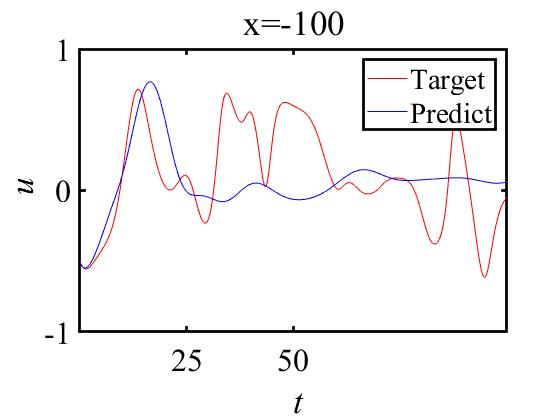
\includegraphics[width=.3\textwidth]{x=-100.jpg}
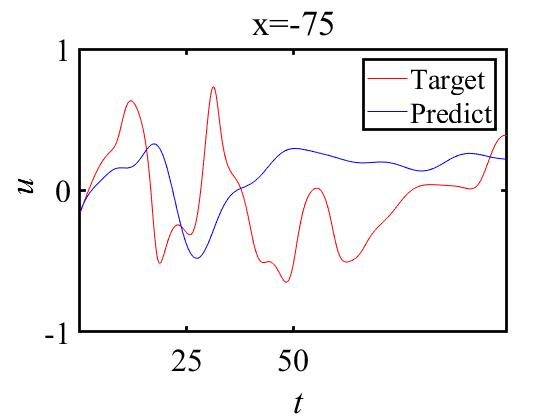
\includegraphics[width=.3\textwidth]{x=-75.jpg}
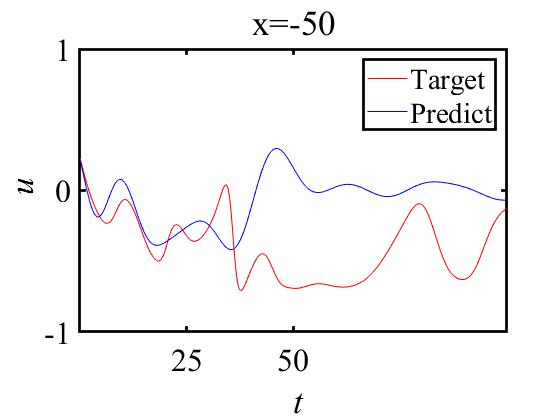
\includegraphics[width=.3\textwidth]{x=-50.jpg}
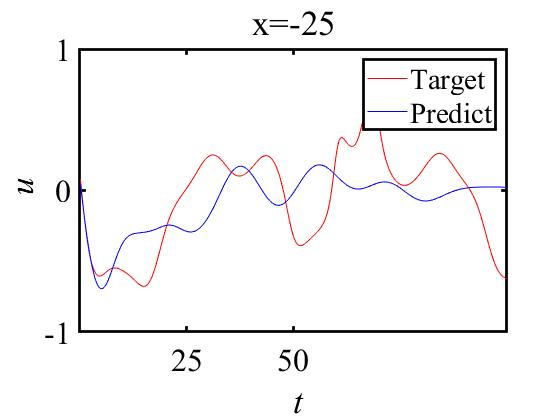
\includegraphics[width=.3\textwidth]{x=-25.jpg}
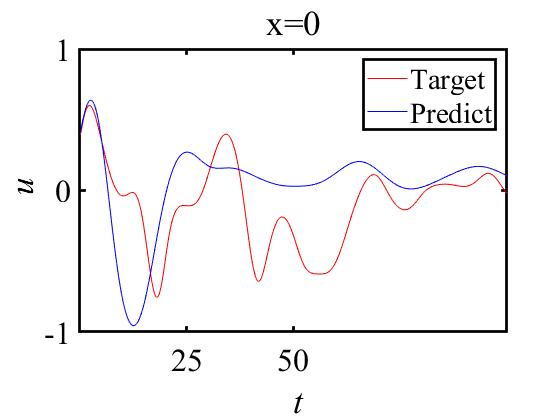
\includegraphics[width=.3\textwidth]{x=0.jpg}
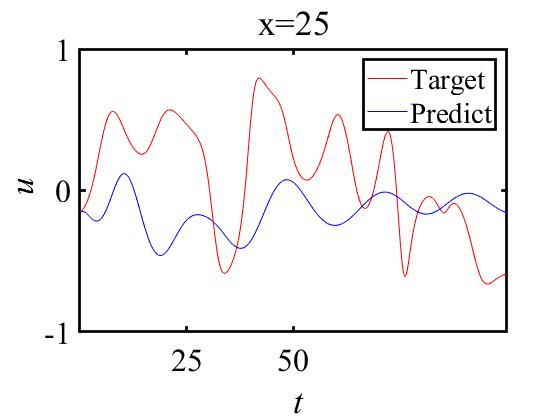
\includegraphics[width=.3\textwidth]{x=25.jpg}
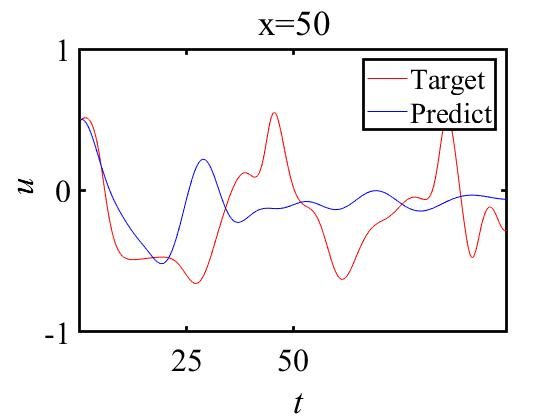
\includegraphics[width=.3\textwidth]{x=50.jpg}
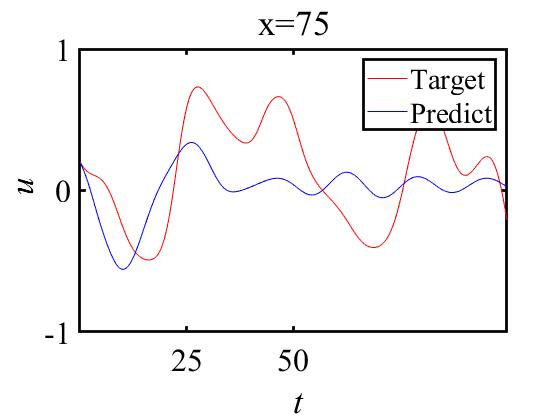
\includegraphics[width=.3\textwidth]{x=75.jpg}
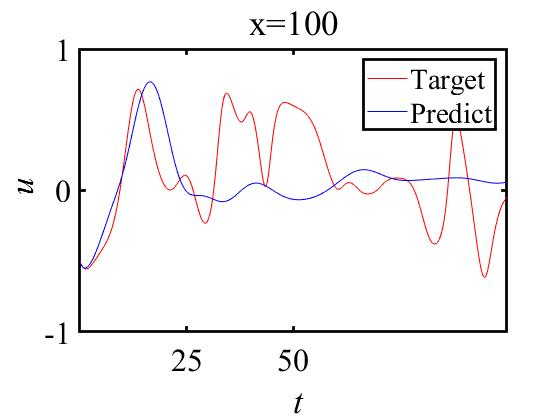
\includegraphics[width=.3\textwidth]{x=100.jpg}
\end{center}
\caption{$x$の25刻みごとの元の時系列と予測結果}%図名
\label{fig:x25}
\end{figure}
この結果からうまく予測できている位置とうまく予測できていない位置があることがわかる.予測がうまくいっている位置では,$t=0\sim20$の200点程度までは予測できていることがわかる.\\
\ 以上の結果から今後の課題として,より予測がうまくいくように学習数や中間層を大きくし予測の精度を上げる,$W_{in},W_{out}$の分布や値の範囲を変える,入力値の刻み幅,時間を変える,減衰してしまうことから$W_{out}$の行列の固有値が1より小さいことが考えられるので正方行列以外で固有値を求める方法を考え,実行する,入力値を最適な時間遅れさせた複数の値にするなどを行う必要がある.

\newpage
\section{今後の予定}
火炎のKS方程式の導出\\
\ or\\
\ スペクトル法\\
\ RCの改善


%\begin{figure}[H]%[h]は記述したところ。[t]はそのページの上端。[t]はそのページの下端、[p]はページいっぱい
%\begin{center}
%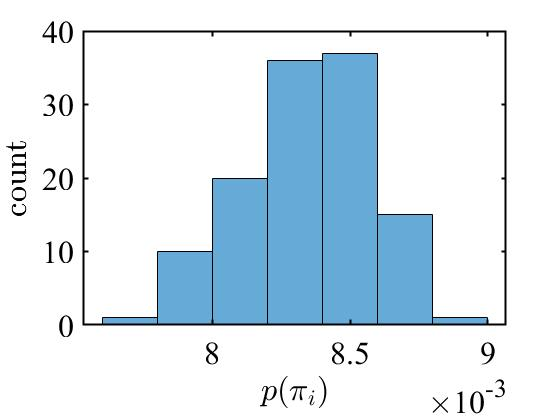
\includegraphics[width=.4\textwidth]{kadai3_histo.jpg}
%\end{center}
%\caption{課題3のヒストグラム(生成数は$100000$)}%図名
%\label{fig:kadai3_3}
%\end{figure}

%チェビシェフの不等式の置き換えの大数の弱法則から,
%\begin{equation}
%P(|\overline{X}_n-\mu|\ge \epsilon) \le \dfrac{\sigma^2}{n \epsilon^2}
%\end{equation}
%となる.ここでの$\overline{X}_n$はサンプルデータ$n$までの平均値(標本),$\mu$は理論的に考えられる平均値,$\epsilon$は許容誤差の大きさ,$\sigma$は標本データの分散である.




%$A^1$\cite{aaa}%参考文献



%\begin{itemize}
%\item アイテムコード1\\
%\item アイテムコード2\\
%\item アイテムコード3\\
%\item アイテムコード4\\
%\item アイテムコード5\\
%\end{itemize}


%\begin{figure}[H]%[h]は記述したところ。[t]はそのページの上端。[t]はそのページの下端、[p]はページいっぱい
%\begin{center}
%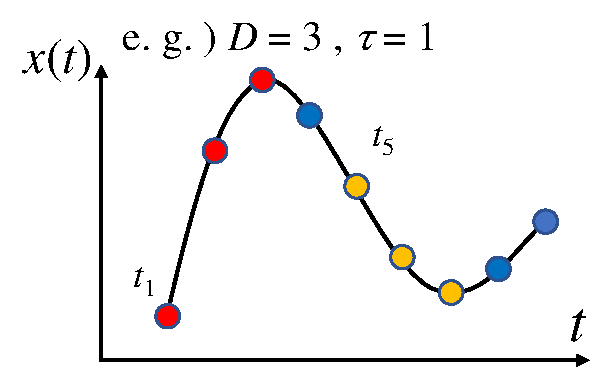
\includegraphics[width=.4\textwidth]{crop_PE1ver2.pdf} 
%\end{center}
%\caption{時系列$ x(t) $}%図名
%\label{fig:PE1}%fig図tb表
%\end{figure}

%\begin{eqnarray}
%\left\{%%{を作る
%\begin{array}{l}%l,llでは、lのときすべて{}の中の式のとき、{}の中にないものがあるならこっち
%\end{array}
%\right.
%\end{eqnarray} 

%式(8a)みたいなのができるぞ式の中で式番号振れるぞ
%\begin{subequations}
%\begin{align}
%a  &= b  & c  &= d  & e  &= f \label{eq:aaaa}\\
%a' &= b' & c' &= d' & e' &= f'\label{eq:bbbb}
%\end{align}
%\label{eq:cccc}
%\end{subequations}
%式(\ref{aaaa}),式(\ref{bbbb}),式(\ref{cccc})


\begin{thebibliography}{9999}%参考文献
\bibitem{all}%参考文献citeするぞ
M. Pradas, G.A. Pavliotis, S. Kalliadasis, D.T. Papageorgiou and D. Tseluiko,"Additive noise
effects in active nonlinear spatially extended systems", European Journal of Applied Mathematics.
23, pp 563$\sim$591 doi:10.1017/S0956792512000125(2012)
%\bibitem{re}
%カオス・フラクタル\ 講義ノート\ \#8,\url{https://ocw.hokudai.ac.jp/wp-content/uploads/2016/01/ChaosFractal-2011-Note-08.pdf}
%\bibitem{wgn}%参考文献citeするぞ
%ホワイトガウスノイズサンプルの生成-MATLAD wgn,\url{https://jp.mathworks.com/help/comm/ref/wgn.html}
%\bibitem{mutual}
%相互情報量の意味とエントロピーとの関係 | 高校数学の美しい物語,\url{https://mathtrain.jp/mutualinfo}
%\bibitem{net}
%複雑ネットワーク:統計物理学の視点,\url{http://mercury.yukawa.kyoto-u.ac.jp/~bussei.kenkyu/pdf/03/1/9999-031210.pdf}
\end{thebibliography}

%\newpage



\end{document}